\documentclass[english,12pt]{article}
\usepackage[T1]{fontenc}
\usepackage[latin9]{luainputenc}
\usepackage{babel}
\usepackage{array}
\usepackage{float}
\usepackage{amstext}
\usepackage{amssymb}
\usepackage{graphicx}
\usepackage{upgreek}
\usepackage{cite}
\usepackage{titlesec}
\usepackage{pgfgantt}
\usepackage{pgfgantt}
\usepackage{graphicx}
\usepackage{xcolor}
\usepackage{pdfpages}

\setcounter{tocdepth}{4}
\setcounter{secnumdepth}{4}

\titleformat{\paragraph}
{\normalfont\normalsize\bfseries}{\theparagraph}{1em}{}
\titlespacing*{\paragraph}
{0pt}{3.25ex plus 1ex minus .2ex}{1.5ex plus .2ex}


\usepackage[unicode=true,pdfusetitle,
 bookmarks=true,bookmarksnumbered=false,bookmarksopen=false,
 breaklinks=false,pdfborder={0 0 1},backref=false,colorlinks=false] {hyperref}

% copying some latex magic from Yuval
\usepackage{xspace}
\usepackage{color}
\newif\ifNotes\Notestrue
\newcommand{\swallow}[1]{}
\ifNotes
  \newcommand{\colorcomment}[2]{\leavevmode\unskip\space{\color{#1}[#2]}\xspace}
\else
  \newcommand{\colorcomment}[2]{\leavevmode\unskip\relax}
\fi
\newcommand{\taggedcolorcomment}[3]{\colorcomment{#1}{\textbf{#2}: #3}}
\newcommand{\todo}[1]{\colorcomment{red}{TODO: #1}}
\newcommand{\refs}{\colorcomment{red}{REFS}}
\newcommand{\yossi}[1]{\taggedcolorcomment{green}{Yossi}{#1}}
\newcommand{\amit}[1]{\taggedcolorcomment{blue}{Amit}{#1}}



% source: https://tex.stackexchange.com/a/74782
\newcommand\dblquote[1]{\textquotedblleft #1\textquotedblright}
\newcommand\textbfit[1]{\textbf{\textit{#1}}}


\makeatletter

%%%%%%%%%%%%%%%%%%%%%%%%%%%%%% LyX specific LaTeX commands. % Because html
%converters don't know tabularnewline
\providecommand{\tabularnewline}{\\}
%% A simple dot to overcome graphicx limitations
\newcommand{\lyxdot}{.}


%%%%%%%%%%%%%%%%%%%%%%%%%%%%%% User specified LaTeX commands.
\usepackage{graphicx}

\makeatother

\begin{document}
\begin{titlepage}

\newcommand{\HRule}{\rule{\linewidth}{0.5mm}} 
% Defines a new command for the horizontal lines, change thickness here

\center % Center everything on the page
 

%----------------------------------------------------------------------------------------
%	LOGO SECTION
%----------------------------------------------------------------------------------------


\includegraphics[scale=0.025]{images/bgu.png}\\[1cm] 


 
%----------------------------------------------------------------------------------------

%----------------------------------------------------------------------------------------
%	HEADING SECTIONS
%----------------------------------------------------------------------------------------

% Name of your university/college 
\textsc{\LARGE Ben-Gurion University of the Negev}\\[1.5cm] 

\textsc{\Large Faculty of Engineering Science}\\[0.5cm] 

% Major heading such as course name 
\textsc{\large Department of Software and Information Systems
Engineering}\\[0.5cm] 

% Minor heading such as course title 
\textsc{\large Project in Offensive Artificial Intelligence Course}\\[0.5cm] 

% Minor heading such as course title

%----------------------------------------------------------------------------------------
%	TITLE SECTION
%----------------------------------------------------------------------------------------

\HRule \\[0.4cm]
{ \huge \bfseries OAI Final Project - Robustness of Real Time Deepfakes } \\[0.4cm] 
% Title of your document 
\HRule \\[1.5cm]
 
%----------------------------------------------------------------------------------------
%	AUTHOR SECTION
%----------------------------------------------------------------------------------------

\begin{minipage}{0.4\textwidth}
\begin{flushleft} \large \emph{Author:}\\
Amit Kama % Your name
\end{flushleft}
\end{minipage}
~
\begin{minipage}{0.4\textwidth}
\begin{flushright} \large \emph{Author:} \\
Oren Shvartzman % Your Name
\end{flushright}
\end{minipage}\\[3cm]

% \begin{minipage}{0.4\textwidth}
% \begin{flushleft} \large \emph{Author:}\\
% Barak Yacouel % Your name
% \end{flushleft}
% \end{minipage}
% ~
% \begin{minipage}{0.4\textwidth}
% \begin{flushleft} \large \emph{ }\\
%   % Your name
% \end{flushleft}
% \end{minipage}\\[2cm]
    
% If you don't want a supervisor, uncomment the two lines below and remove the
% section above \Large \emph{Author:}\\
% John \textsc{Smith}\\[3cm] % Your name

%----------------------------------------------------------------------------------------
%	DATE SECTION
%----------------------------------------------------------------------------------------

{\large \today}\\[3cm] 
% Date, change the \today to a set date if you want to be precise


\vfill % Fill the rest of the page with whitespace

\end{titlepage}

\pagebreak{}


\tableofcontents{}

\pagebreak{}


\section{Introduction} \label{introduction}

% Deepfakes and deepfakes in recent years
Deepfake is a general term that encompasses the use of deep learning algorithms in order to create
synthetic media, in which one subject in an existing visual and/or audio content is usually replaced
with another's likeness. While fraudulent content has been around for some time, recent advances in
machine vision have posed a major threat to the trust and transparency of the media. Using powerful
machine-learning and deep-learning techniques, deepfakes can now manipulate or generate visual and
audio content that can be more easily misleading.

In recent years, deepfakes have garnered widespread attention for their uses in spreading fake news,
committing financial fraud, creating pornographic materials, and many other disturbing uses. This has
led to a significant need to identify and restrict their use.

% First Order Model
Ever since the introduction of deepfakes, researchers in deep learning have increasingly focused on
this area of research. In particular, they propose methods, as well as practical implementations of
deepfakes is in various fields. Among other methods, in~\cite{DBLP:journals/corr/abs-2003-00196}, Siarohin et al. propose
the first order motion model for image animation. Their framework enables generating a video sequence,
in which an object in a source image is animated according to the motion of a driving video, without
using any annotation or prior information about the specific object to animate. According to them,
once trained on a set of videos depicting objects of the same category, the method can be applied
to any object of it. Based on this method, a number of real time photorealistic avatars have recently
been developed, one of which we will explore in this work.

% It has limitations - drawbacks, that in the literature, there is a growing amount of research dealing with the field.
However, real time avatars are far from perfect, as they are not robust when it comes to edge cases.
This includes facial gestures in the driving video, objects in the source or target media that make it
difficult to identify facial boundaries, and many more.


% Detection (Importance, ways)
Note that these limitations can be create visual glitches and distortions that can be detected with the
naked eye as well as by software, and therefore can be utilized for deepfakes detection. This observation
drives a growing amount of research dealing with those inaccuracies for dual use -- correcting them in
order to improve the deepfakes' credibility, or exploiting them to distinguish deepfakes from real content.

% What will be in the report
In this work, we evaluate the robustness of real time deepfakes by implementing first order motion
model-based avatarify and examining various edge cases on it. After demonstrating failures in the
implementation, we also provide a method to utilize them for deepfakes detection.


% \pagebreak{}

\section{Methods} \label{methods}

In this section we will briefly introduce the implementation on which our work relies on, and the
First Order Model, on which the Avatarify Python consists of.

% Detailed explanation on First Order Model
\subsection{First Order Motion Model}
% From DBLP:journals/corr/abs-2003-00196
% The method, our plan to evaluate it


%+++++++++++++++++++++++++++++++++++++++++++++++++++++++++++++++++++++++++++++++++++++++++++++++++++++++++++++++++++++++


% FIXME: Do we want to add figures from the paper?
First Order Motion Model for Image Animation

% Abstract

% FIXME: rephrase
In~\cite{DBLP:journals/corr/abs-2003-00196}, Siarohin et al. propose a framework which addresses the problem
of generating a video sequence so that an object in a source image is animated according to the motion of a
driving video, without using any annotation or prior information about the specific object to animate.

Once trained on a set of videos
depicting objects of the same category (e.g. faces, human bodies), our method can be applied to any
object of this class. To achieve this, we decouple appearance and motion information using a self-supervised
formulation. To support complex motions, we use a representation consisting of a set of learned keypoints
along with their local affine transformations. A generator network models occlusions arising during target
motions and combines the appearance extracted from the source image and the motion derived from the driving
video. Our framework scores best on diverse benchmarks and on a variety of object categories.

% From the Introduction
In the literature, most methods tackle this problem by assuming strong priors on the object representation
(e.g. 3D model) [4] and resorting to computer graphics techniques [6, 33]. These approaches can be referred
to as object-specific methods, as they assume knowledge about the model of the specific object to animate.

Recently, deep generative models have emerged as effective techniques for image animation and video
retargeting [2, 41, 3, 42, 27, 28, 37, 40, 31, 21]. In particular, Generative Adversarial Networks (GANs)
[14] and Variational Auto-Encoders (VAEs) [20] have been used to transfer facial expres- sions [37] or
motion patterns [3] between human subjects in videos. Nevertheless, these approaches usually rely on
pre-trained models in order to extract object-specific representations such as keypoint locations.
Unfortunately, these pre-trained models are built using costly ground-truth data annotations [2, 27, 31]
and are not available in general for an arbitrary object category. To address this issues, recently
Siarohin et al. [28] introduced Monkey-Net, the first object-agnostic deep model for image animation.
Monkey-Net encodes motion information via keypoints learned in a self-supervised fash- ion. At test time,
the source image is animated according to the corresponding keypoint trajectories estimated in the driving
video. The major weakness of Monkey-Net is that it poorly models object appearance transformations in the
keypoint neighborhoods assuming a zeroth order model (as we show in Sec. 3.1). This leads to poor generation
quality in the case of large object pose changes (see Fig. 4). To tackle this issue, we propose to use a
set of self-learned keypoints together with local affine transformations to model complex motions. We
therefore call our method a first-order motion model. Second, we introduce an occlusion-aware generator,
which adopts an occlusion mask automatically estimated to indicate object parts that are not visible in the
source image and that should be inferred from the context. This is especially needed when the driving video
contains large motion patterns and occlusions are typical. Third, we extend the equivariance loss commonly
used for keypoints detector training [18, 44], to improve the estimation of local affine transformations.
Fourth, we experimentally show that our method significantly outperforms state-of-the-art image animation
methods and can handle high-resolution datasets where other approaches generally fail. Finally, we release
a new high resolution dataset, Thai-Chi-HD, which we believe could become a reference benchmark for evaluating
frameworks for image animation and video generation.

% FIXME: Add the method

% Conclusions
We presented a novel approach for image animation based on keypoints and local affine transforma- tions. Our
novel mathematical formulation describes the motion field between two frames and is efficiently computed by
deriving a first order Taylor expansion approximation. In this way, motion is described as a set of keypoints
displacements and local affine transformations. A generator network combines the appearance of the source image
and the motion representation of the driving video. In addition, we proposed to explicitly model occlusions in
order to indicate to the generator network which image parts should be inpainted. We evaluated the proposed
method both quantitatively and qualitatively and showed that our approach clearly outperforms state of the art
on all the benchmarks.


%+++++++++++++++++++++++++++++++++++++++++++++++++++++++++++++++++++++++++++++++++++++++++++++++++++++++++++++++++++++++


% Explanation on our proposed method
\subsection{Failures Detection Method}


% \pagebreak{}

\section{Experiments and Results} \label{experiments and results}

In this section we introduce the experiments and results. A detailed explanation of the
visual glitches and distortions that we managed to create and detect is provided, as well
as the results of our proposed method to utilize them for deepfakes detection.

% examples for edge cases on the Avatarify
\subsection{First Order Model Robustness}

\begin{figure}[htb]
  \begin{centering}
      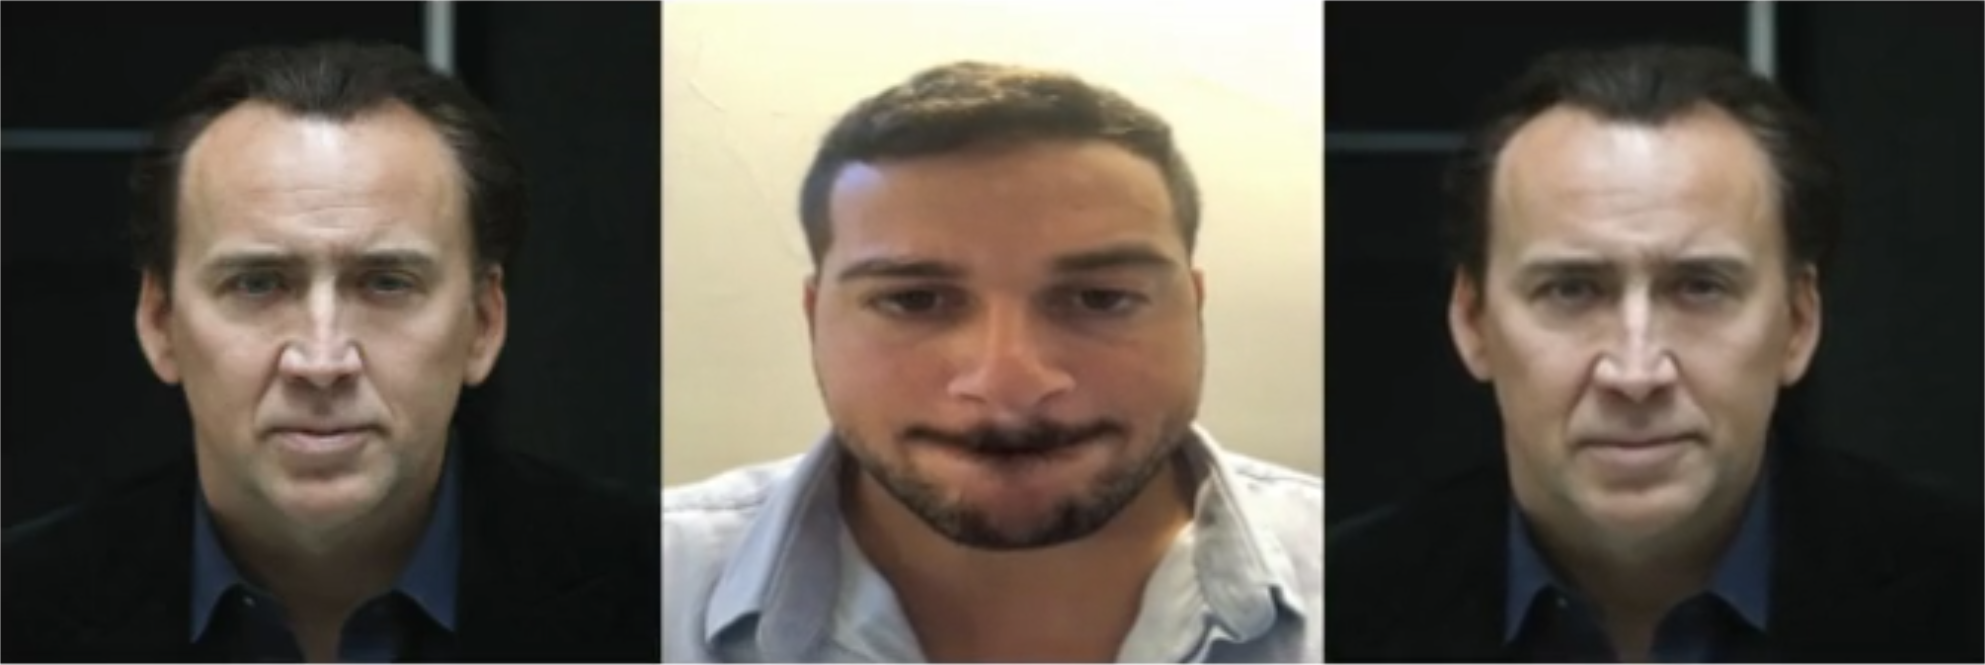
\includegraphics[scale=0.29]{images/‏‏Amit_lips_cage.PNG}
  \par\end{centering}
  \caption{\label{fig:Amit_lips_cage}The effect of...}
\end{figure}

\begin{figure}[htb]
  \begin{centering}
      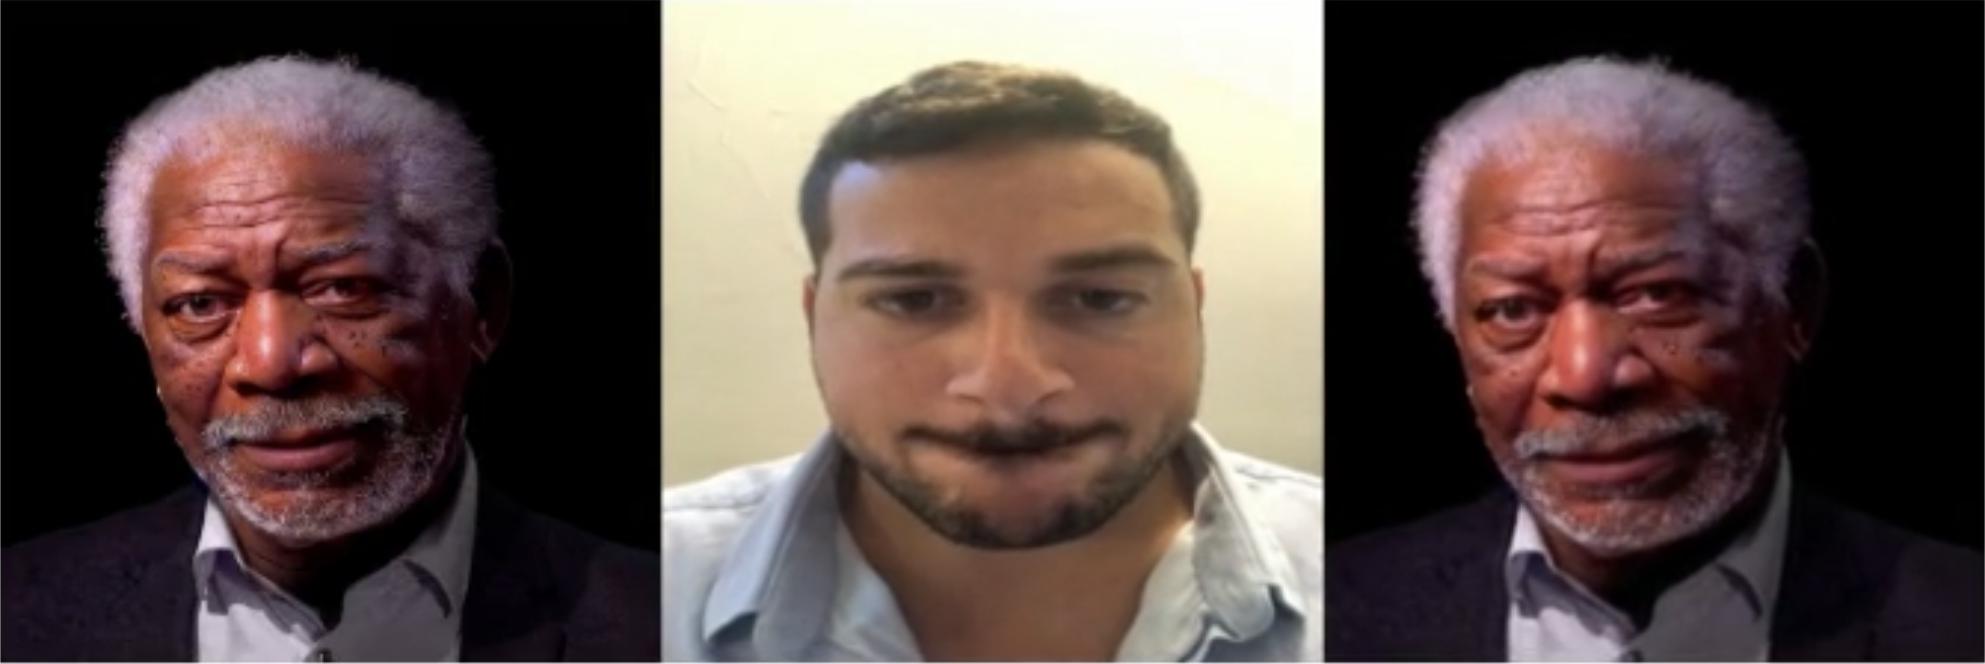
\includegraphics[scale=0.29]{images/‏‏Amit_lips_freeman.PNG}
  \par\end{centering}
  \caption{\label{fig:Amit_lips_freeman}The effect of...}
\end{figure}

\begin{figure}[htb]
  \begin{centering}
      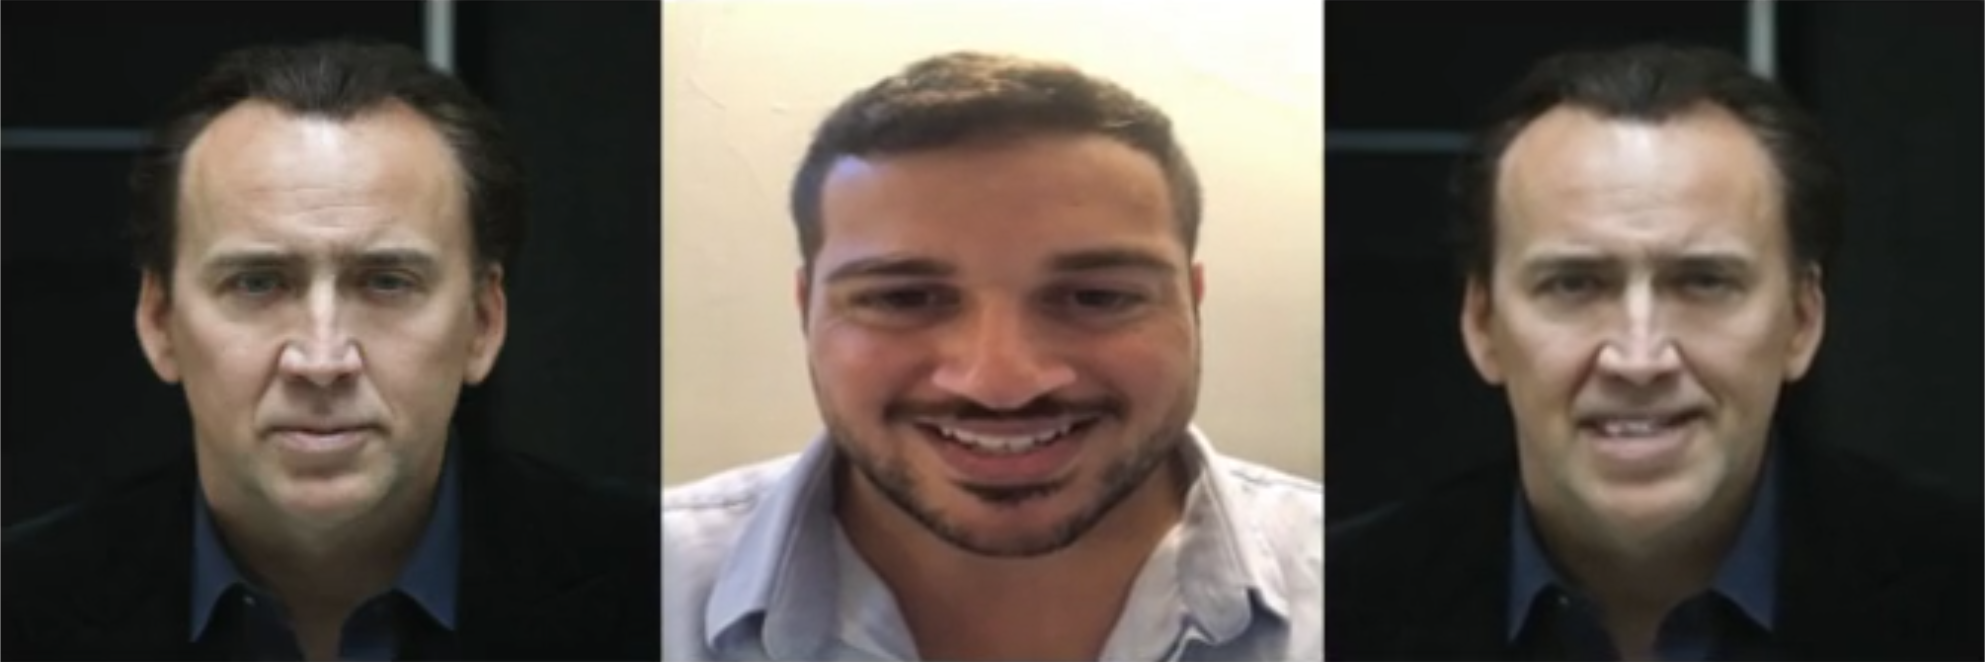
\includegraphics[scale=0.29]{images/‏‏Amit_smile_cage.PNG}
  \par\end{centering}
  \caption{\label{fig:Amit_smile_cage}The effect of...}
\end{figure}

\begin{figure}[htb]
  \begin{centering}
      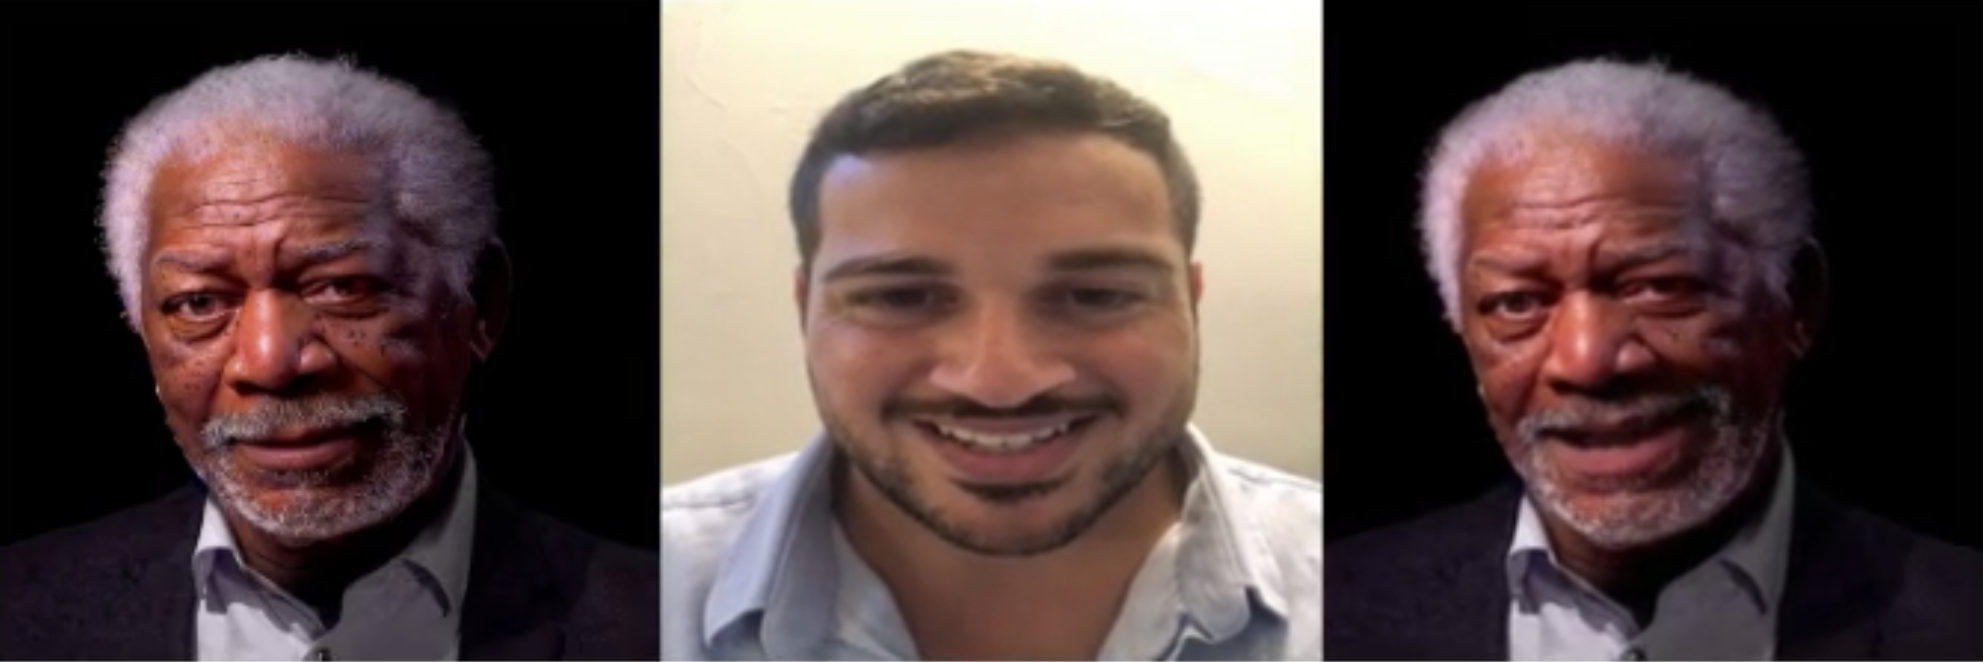
\includegraphics[scale=0.29]{images/‏‏Amit_smile_freeman.PNG}
  \par\end{centering}
  \caption{\label{fig:Amit_smile_freeman}The effect of...}
\end{figure}

\begin{figure}[htb]
  \begin{centering}
      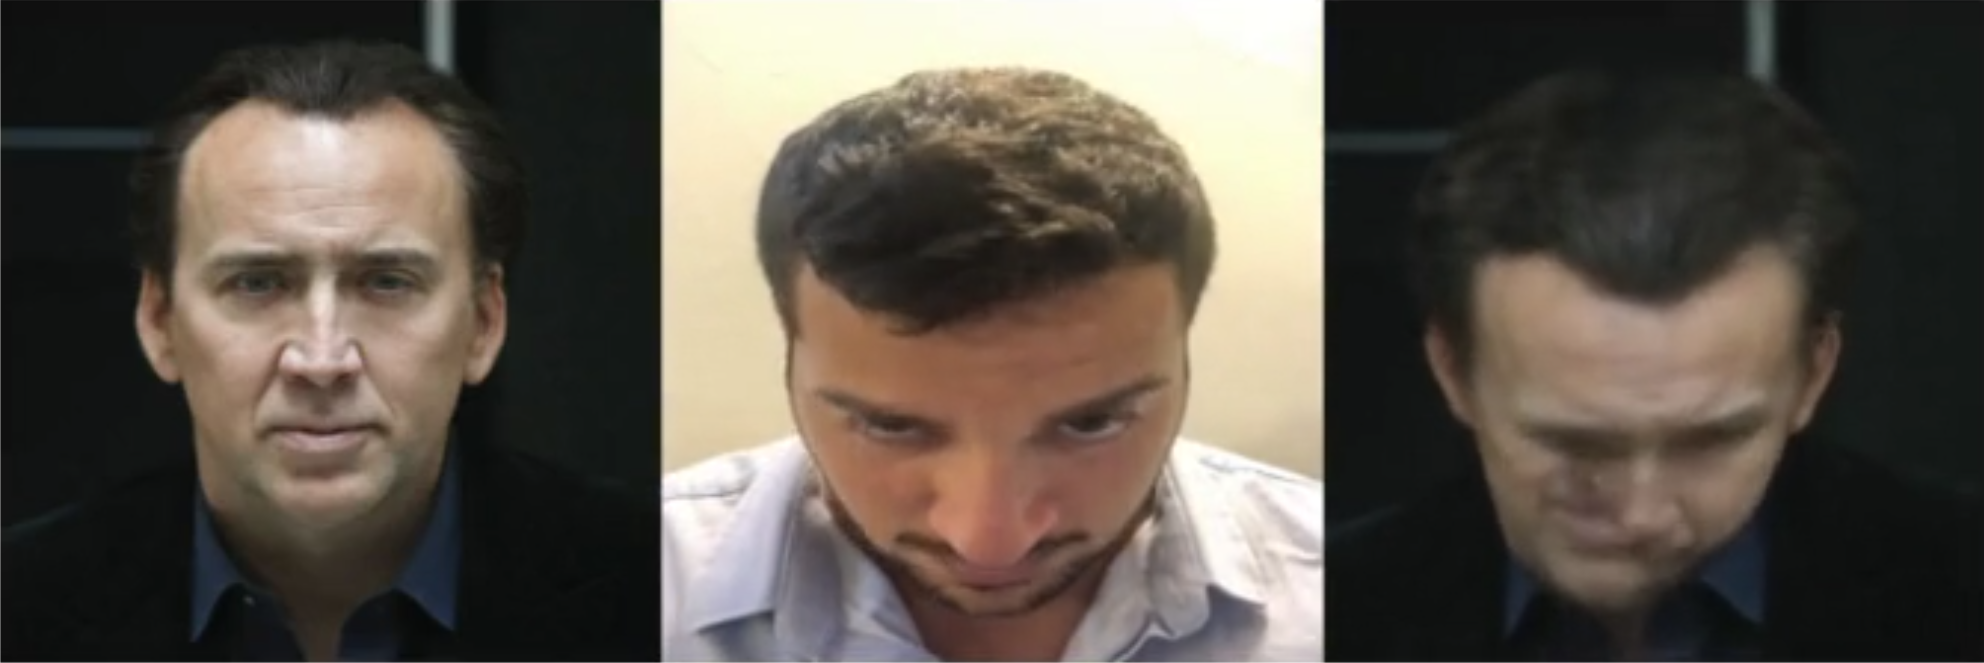
\includegraphics[scale=0.29]{images/‏‏Amit_tilt1_cage.PNG}
  \par\end{centering}
  \caption{\label{fig:Amit_tilt1_cage}The effect of...}
\end{figure}

\begin{figure}[htb]
  \begin{centering}
      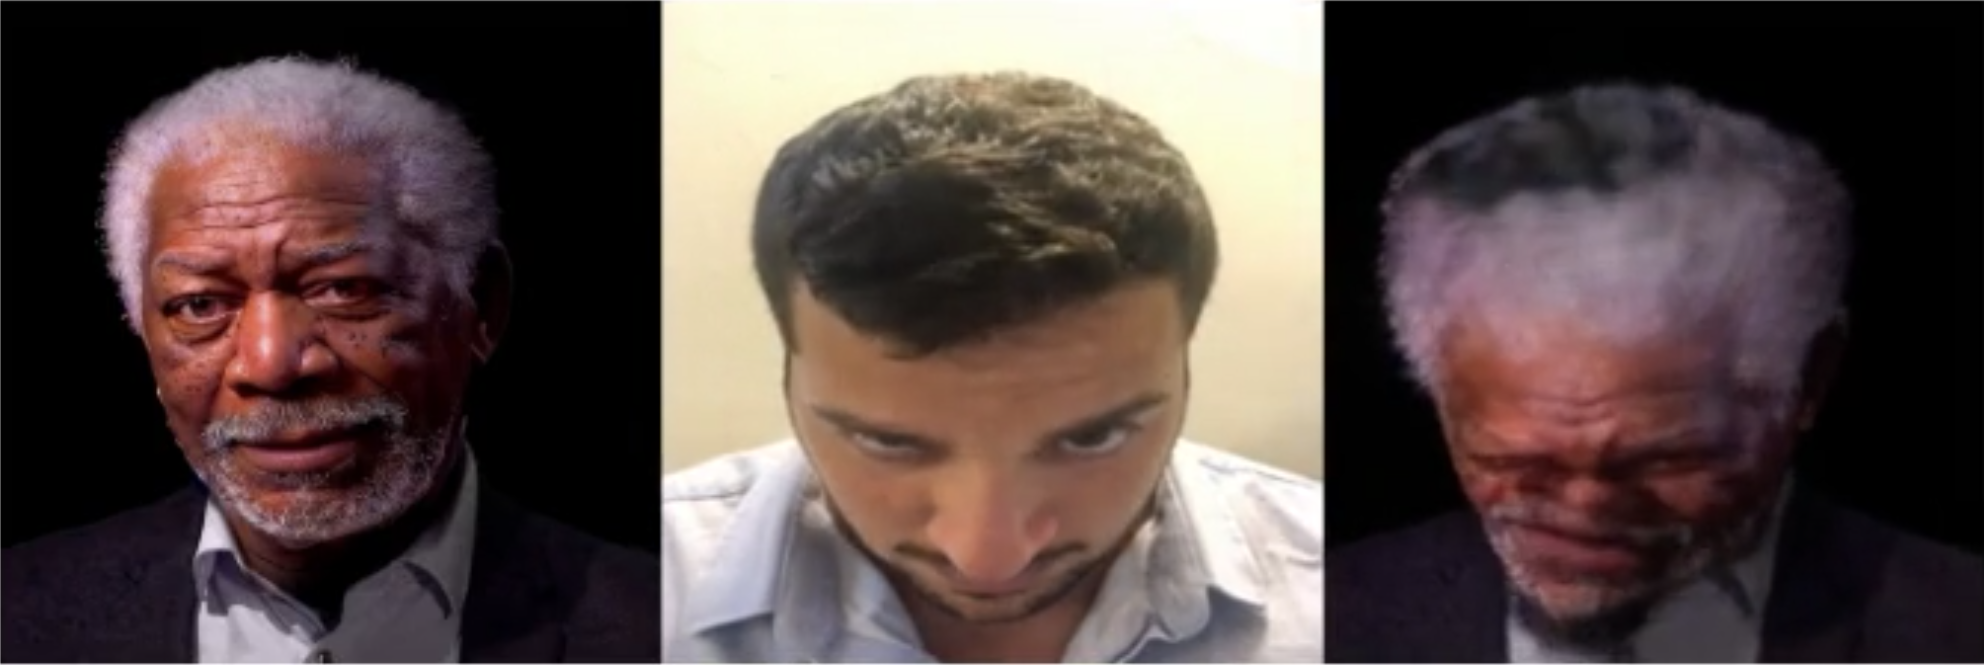
\includegraphics[scale=0.29]{images/‏‏Amit_tilt1_freeman.PNG}
  \par\end{centering}
  \caption{\label{fig:Amit_tilt1_freeman}The effect of...}
\end{figure}

\begin{figure}[htb]
  \begin{centering}
      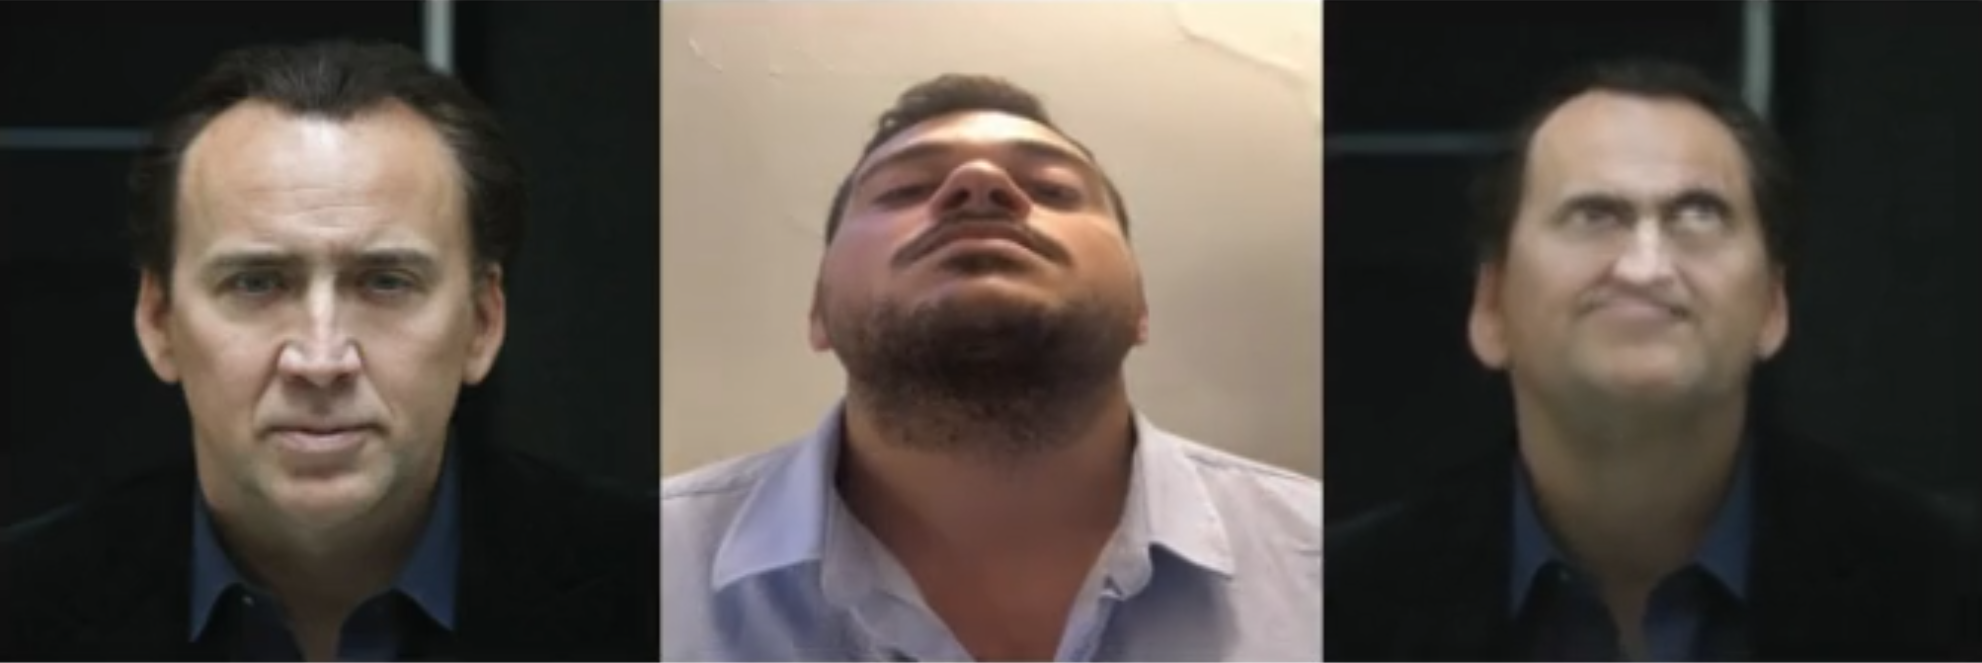
\includegraphics[scale=0.29]{images/‏‏Amit_tilt_cage.PNG}
  \par\end{centering}
  \caption{\label{fig:Amit_tilt_cage}The effect of...}
\end{figure}

\begin{figure}[htb]
  \begin{centering}
      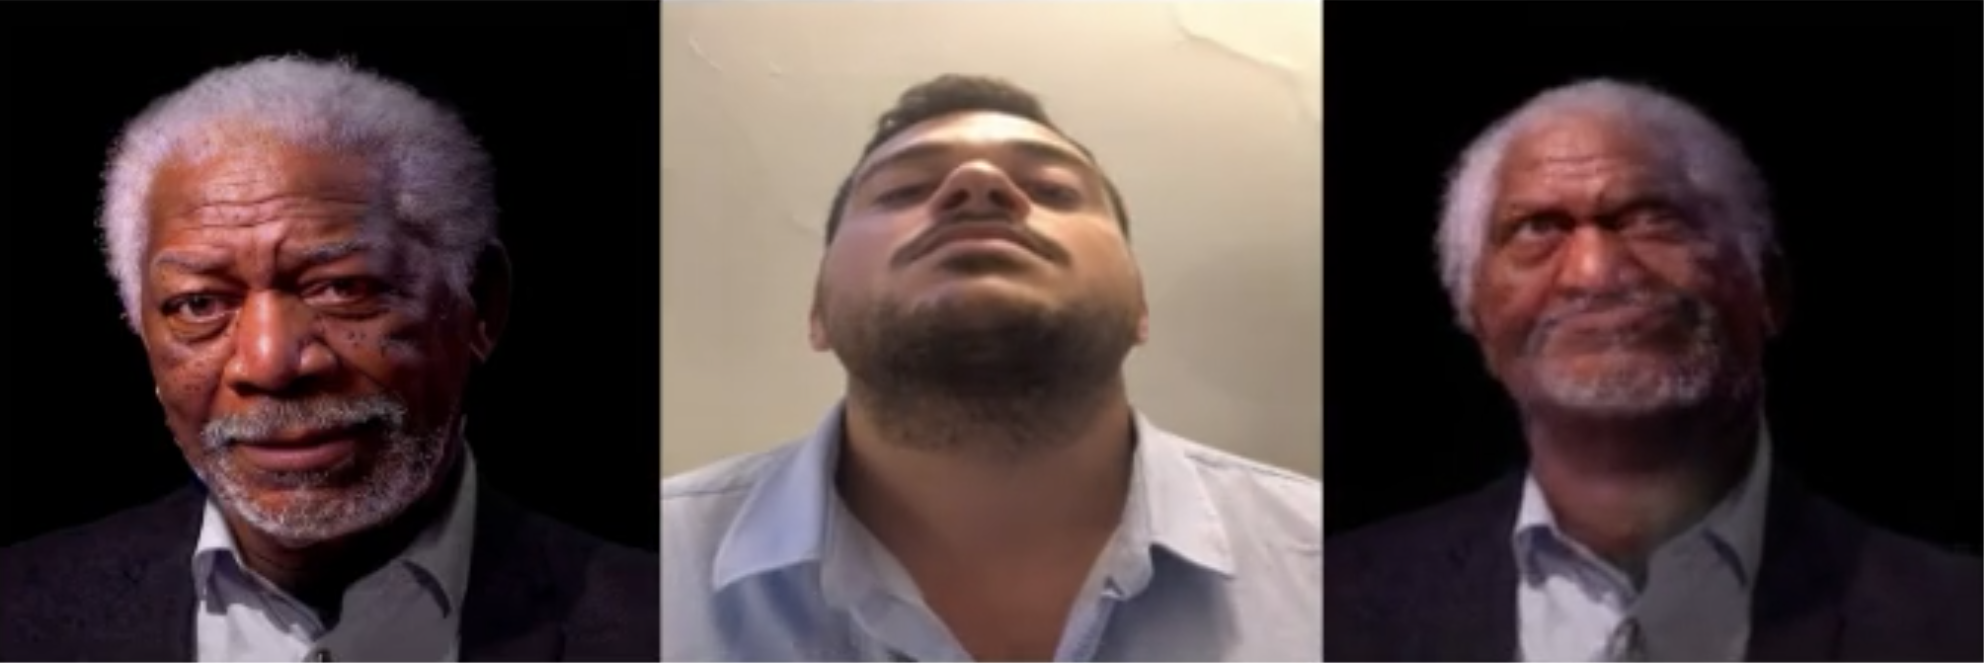
\includegraphics[scale=0.29]{images/‏‏Amit_tilt_freeman.PNG}
  \par\end{centering}
  \caption{\label{fig:Amit_tilt_freeman}The effect of...}
\end{figure}

\begin{figure}[htb]
  \begin{centering}
      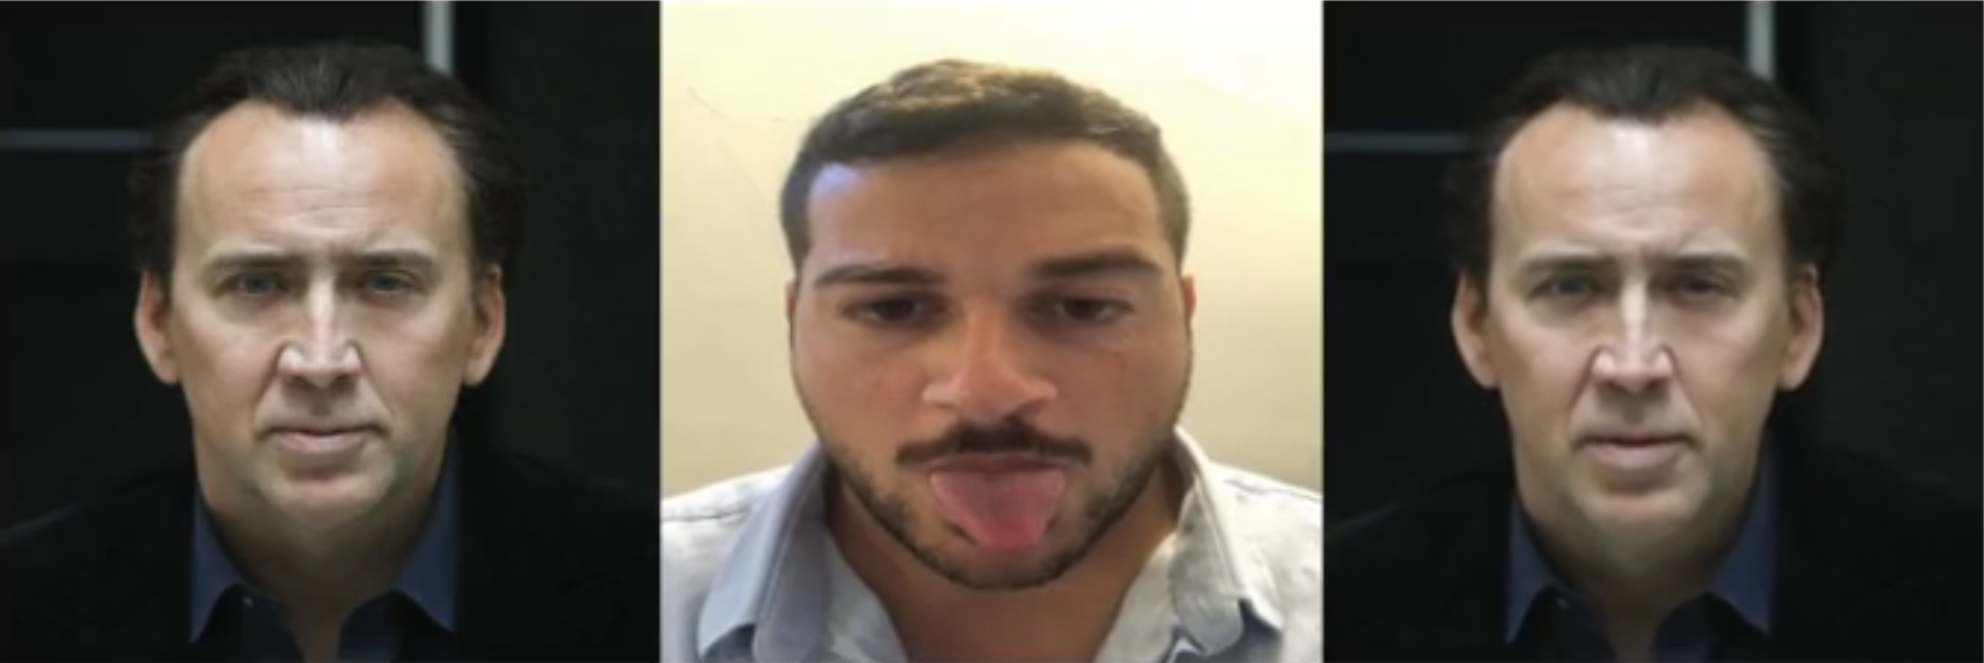
\includegraphics[scale=0.29]{images/‏‏Amit_tongue_cage.PNG}
  \par\end{centering}
  \caption{\label{fig:Amit_tongue_cage}The effect of...}
\end{figure}

\begin{figure}[htb]
  \begin{centering}
      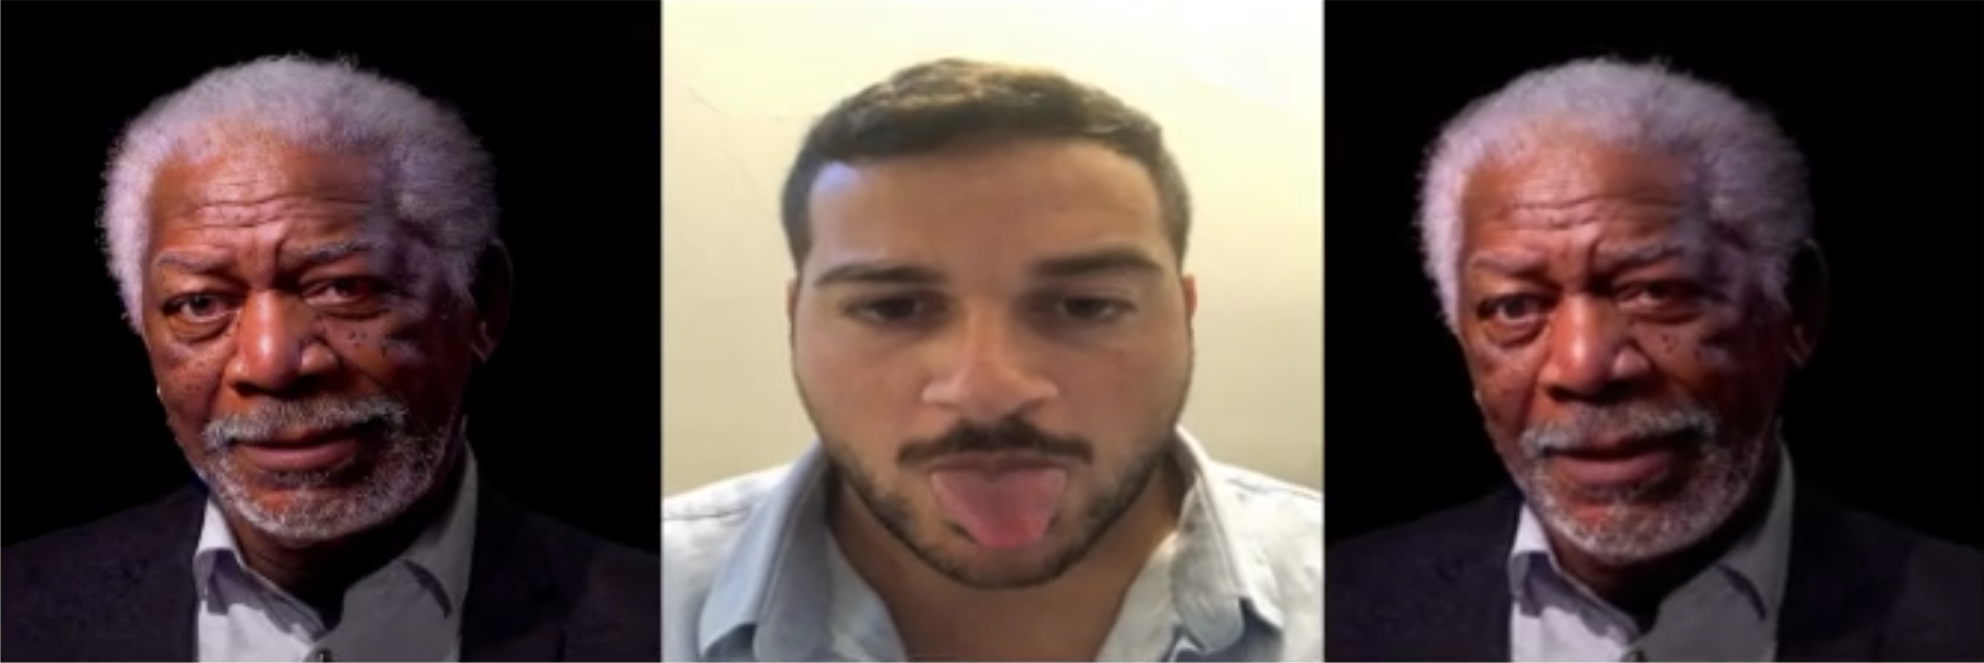
\includegraphics[scale=0.29]{images/‏‏Amit_tongue_freeman.PNG}
  \par\end{centering}
  \caption{\label{fig:Amit_tongue_freeman}The effect of...}
\end{figure}

\begin{figure}[htb]
  \begin{centering}
      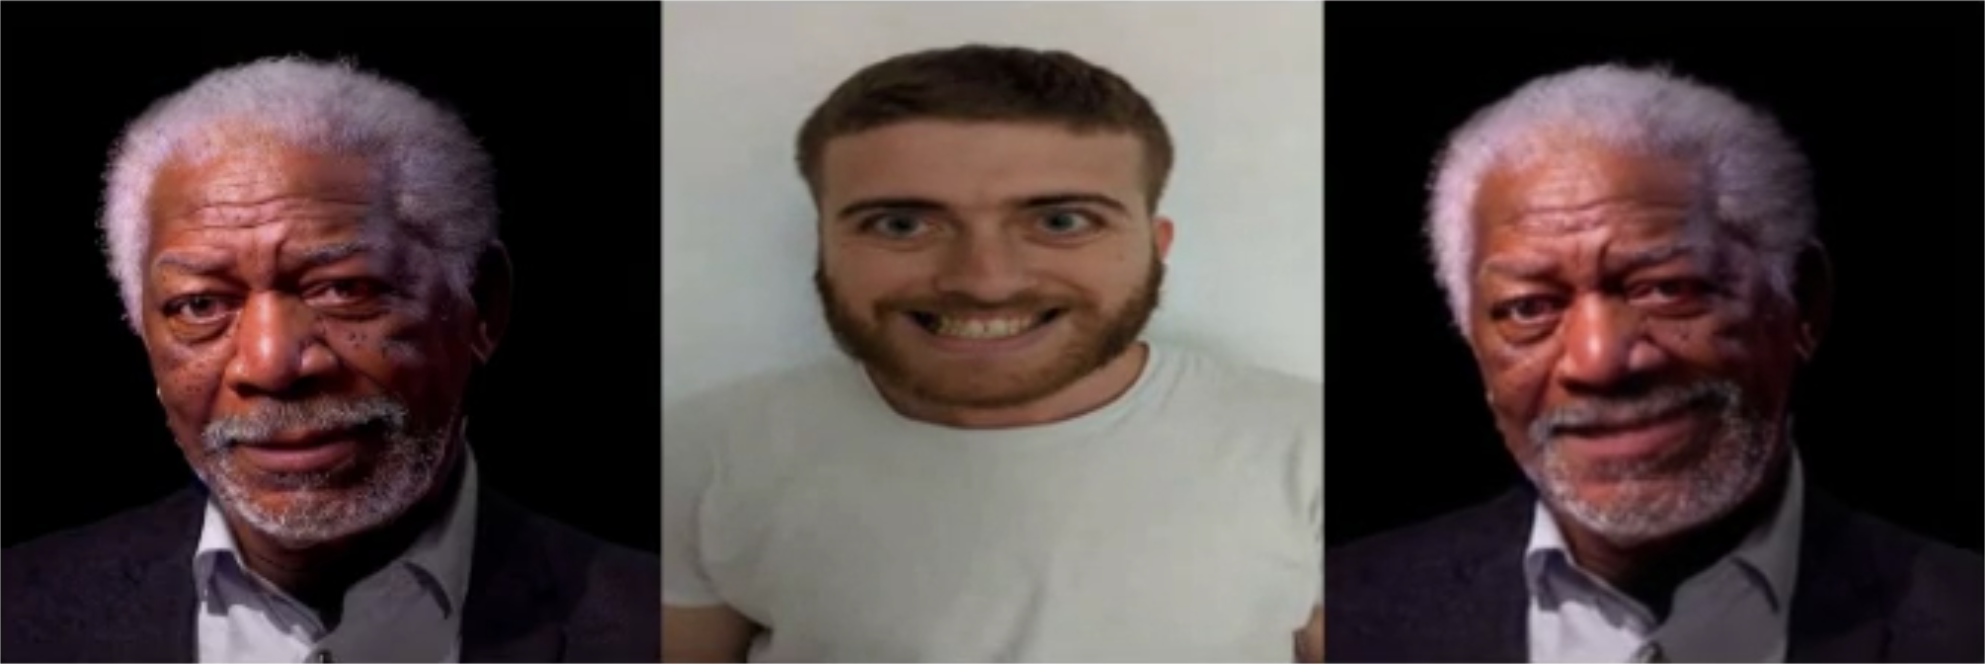
\includegraphics[scale=0.29]{images/Oren_smile_freeman.PNG}
  \par\end{centering}
  \caption{\label{fig:Oren_smile_freeman}The effect of...}
\end{figure}

\begin{figure}[htb]
  \begin{centering}
      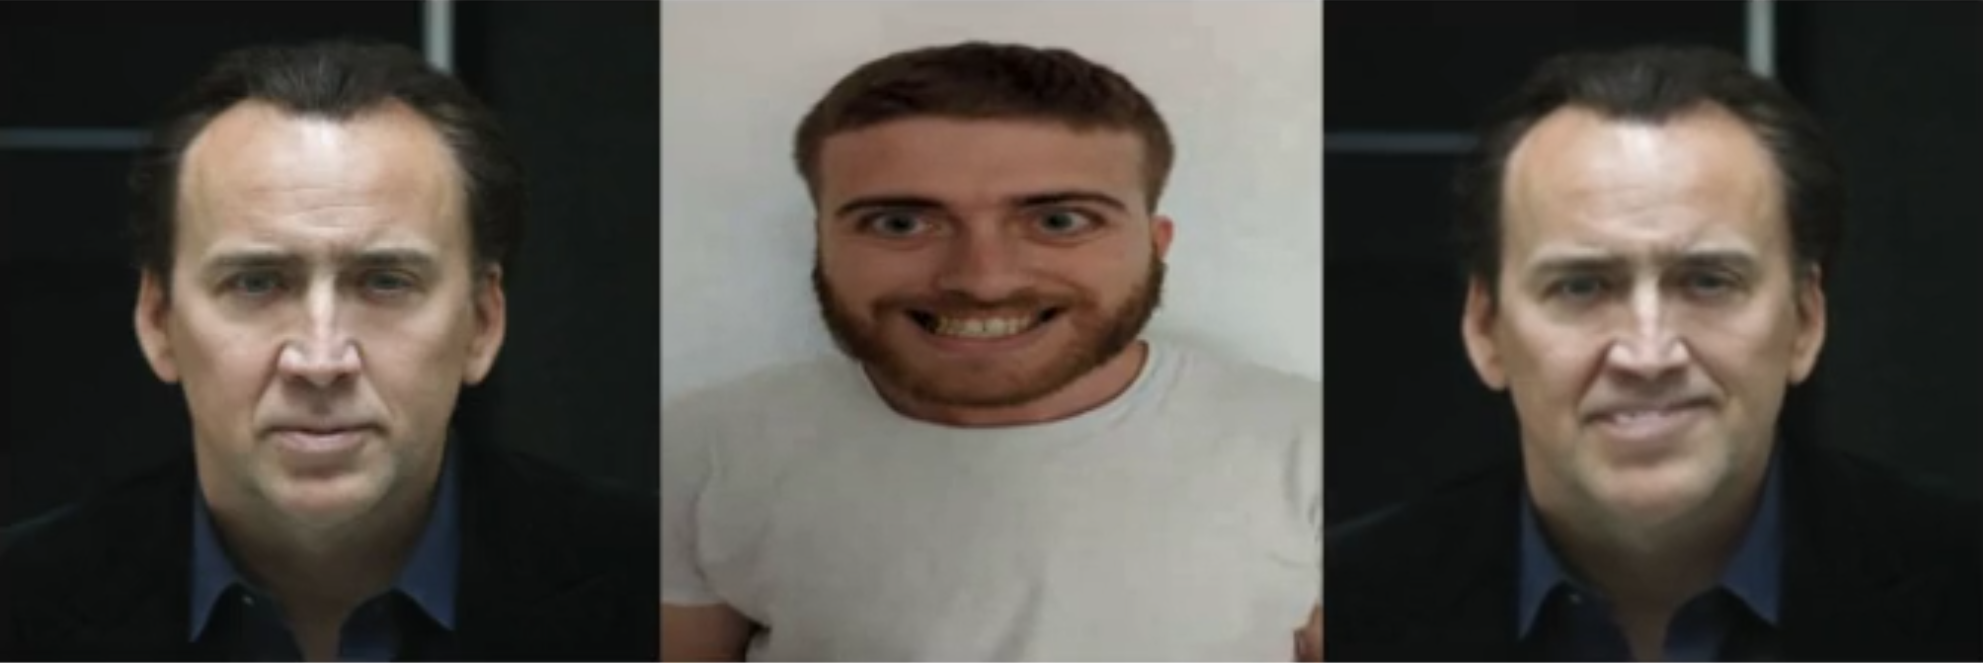
\includegraphics[scale=0.29]{images/‏‏Oren_smile_cage.PNG}
  \par\end{centering}
  \caption{\label{fig:Oren_smile_cage}The effect of...}
\end{figure}

\begin{figure}[htb]
  \begin{centering}
      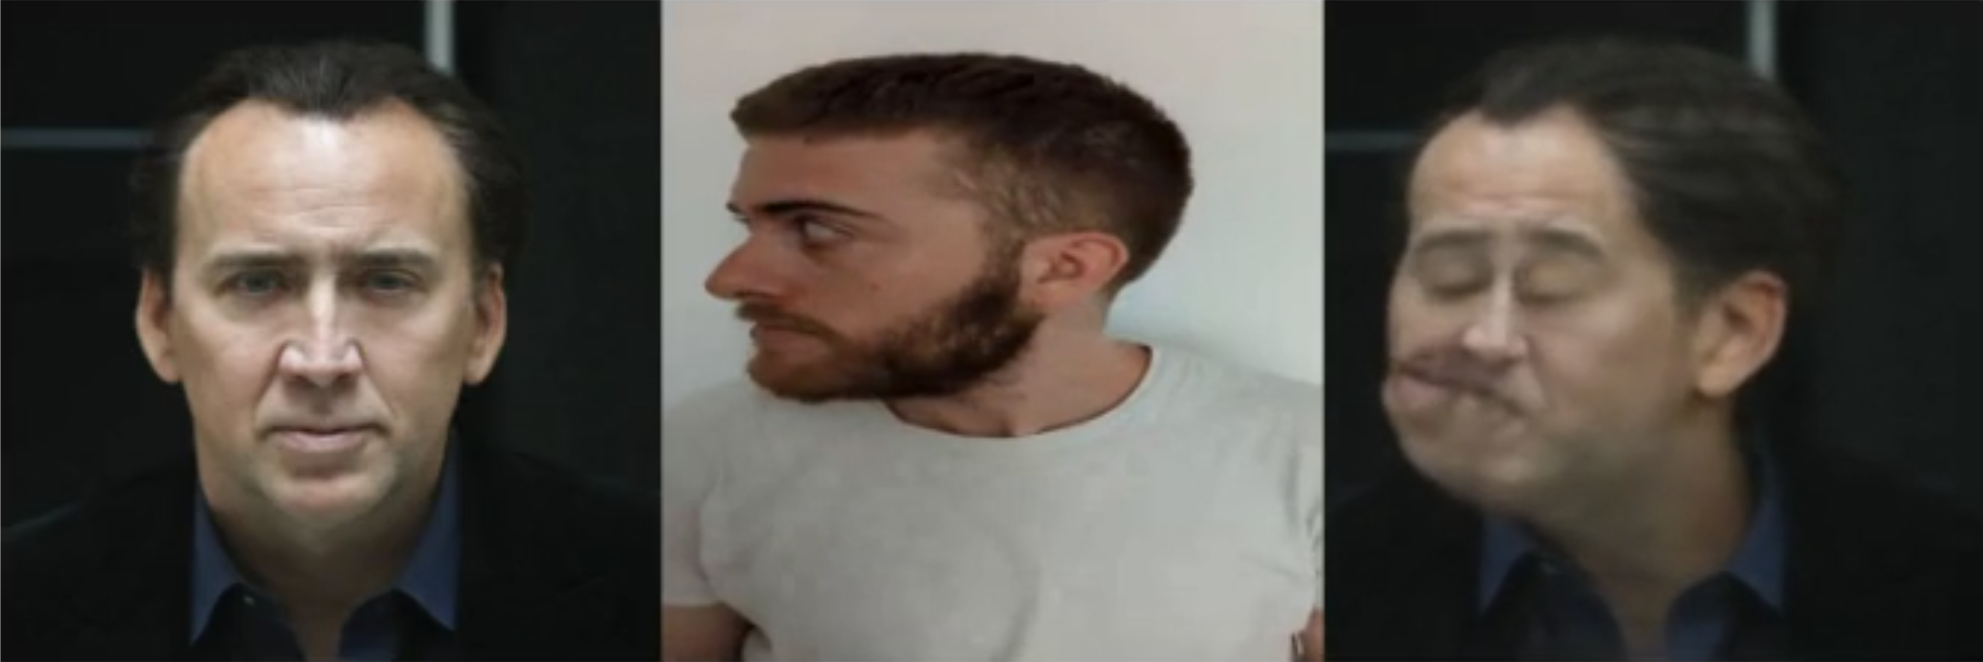
\includegraphics[scale=0.29]{images/Oren_tilt_cage.PNG}
  \par\end{centering}
  \caption{\label{fig:Oren_tilt_cage}The effect of...}
\end{figure}

\begin{figure}[htb]
  \begin{centering}
      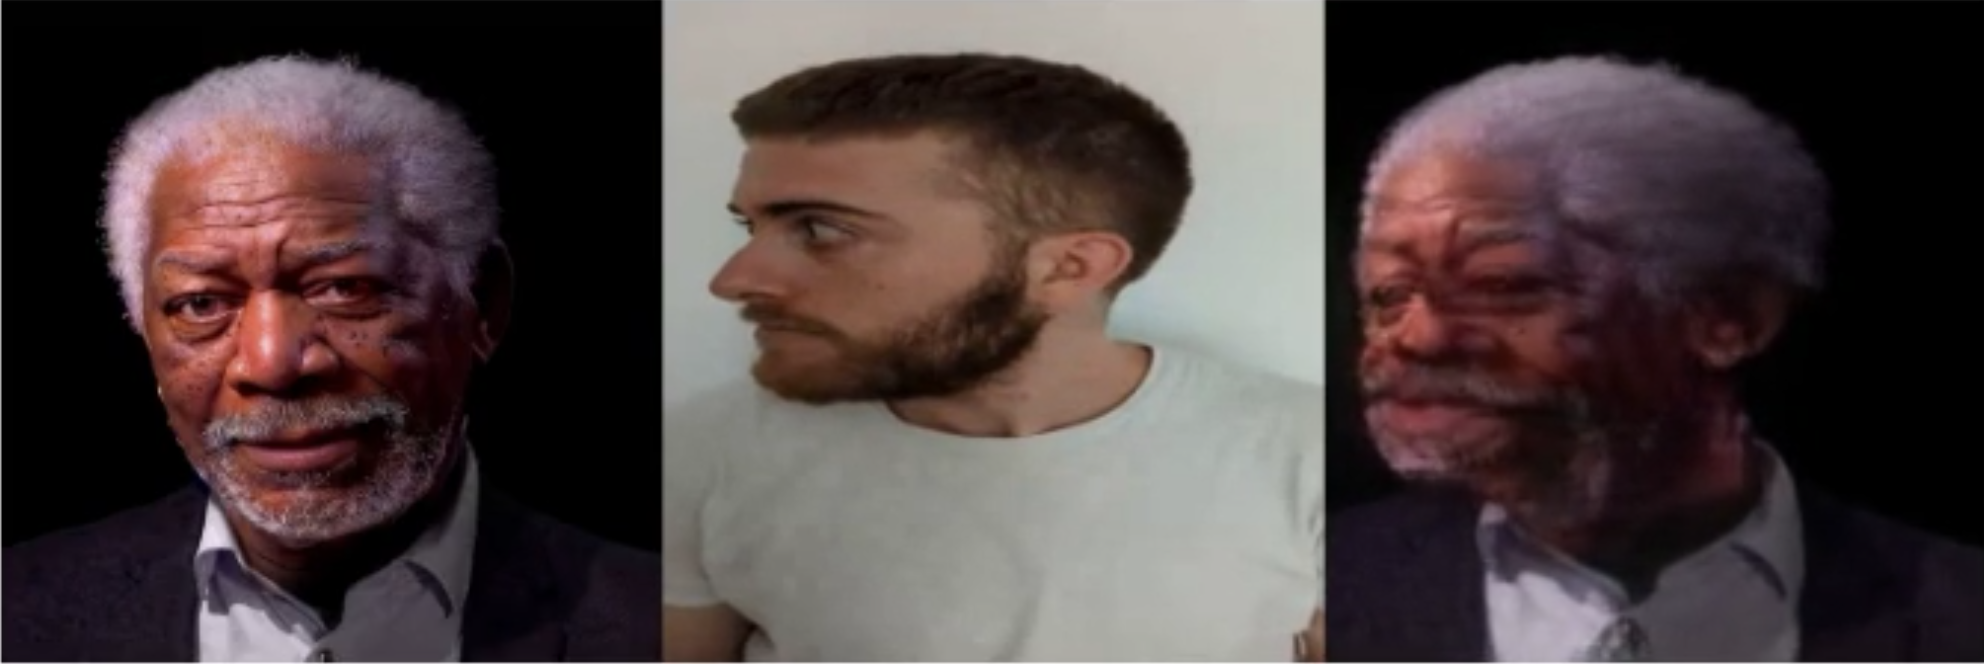
\includegraphics[scale=0.29]{images/Oren_tilt_freeman.PNG}
  \par\end{centering}
  \caption{\label{fig:Oren_tilt_freeman}The effect of...}
\end{figure}

\begin{figure}[htb]
  \begin{centering}
      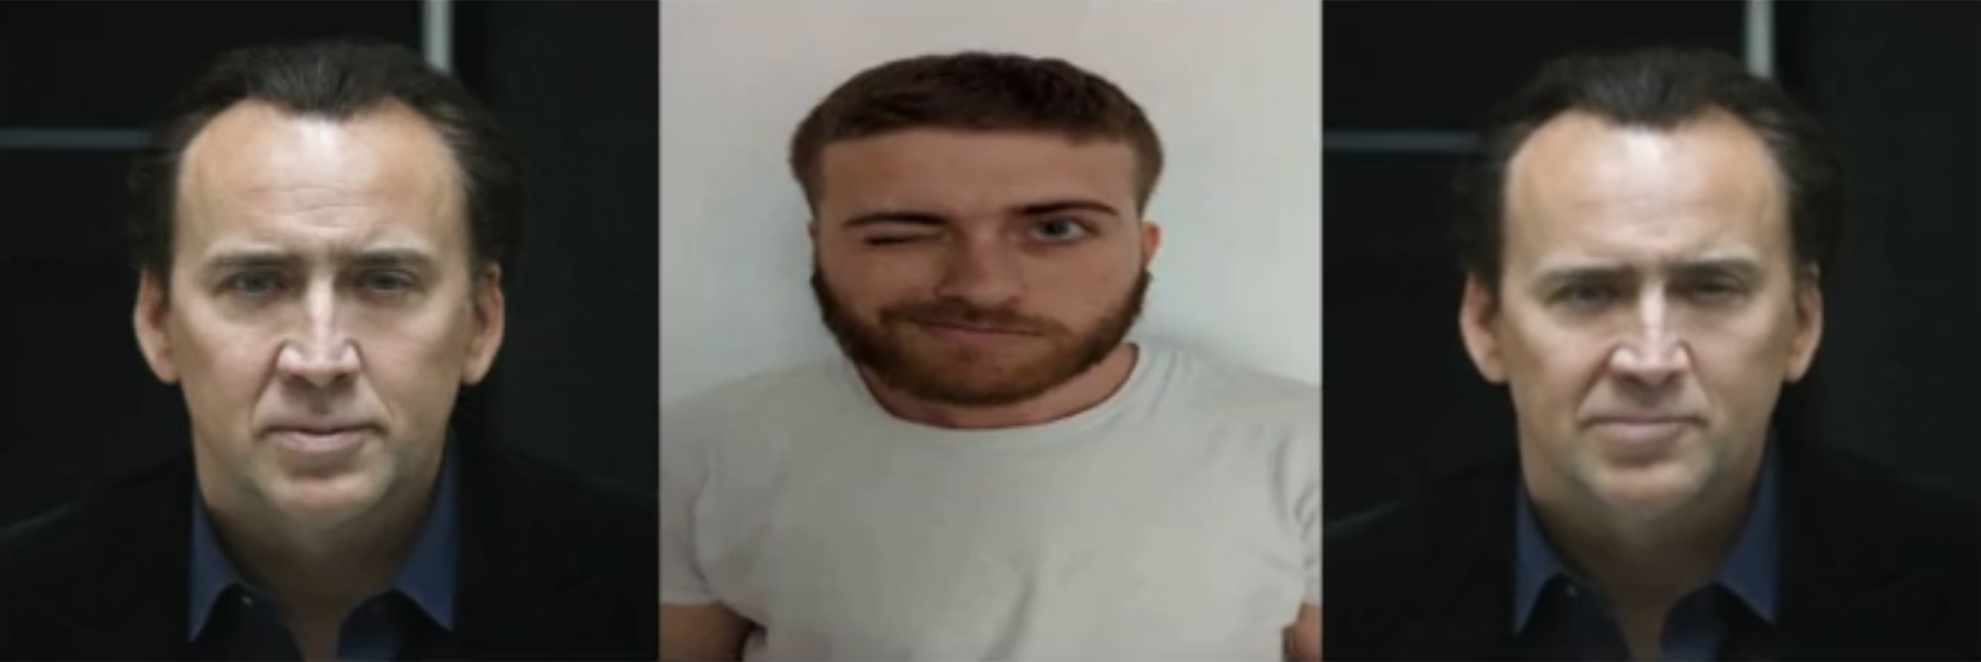
\includegraphics[scale=0.29]{images/Oren_wink_cage.PNG}
  \par\end{centering}
  \caption{\label{fig:Oren_wink_cage}The effect of...}
\end{figure}

\begin{figure}[htb]
  \begin{centering}
      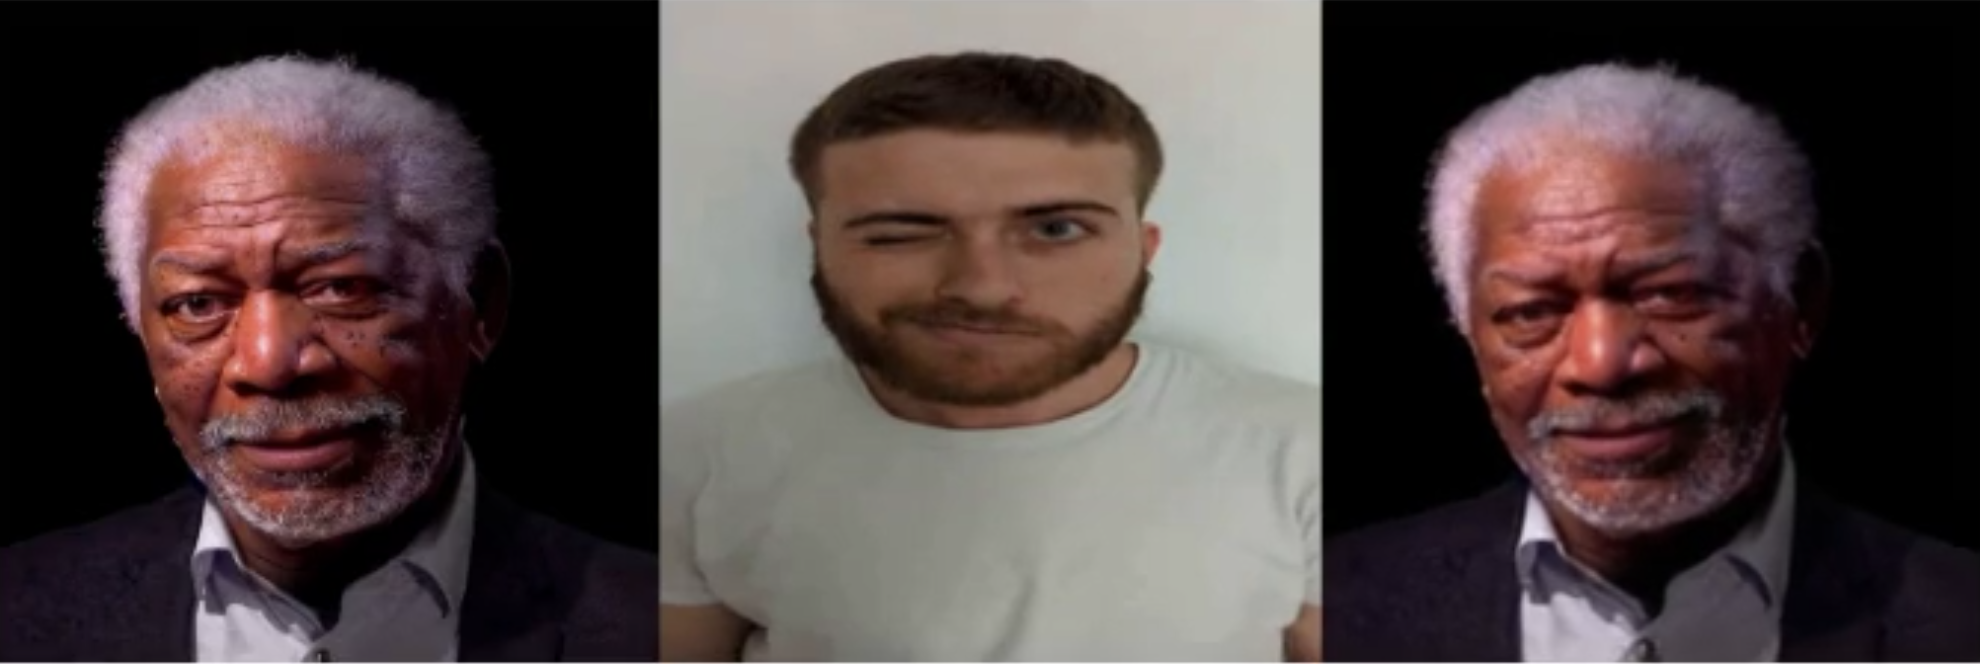
\includegraphics[scale=0.29]{images/Oren_wink_freeman.PNG}
  \par\end{centering}
  \caption{\label{fig:Oren_wink_freeman}The effect of...}
\end{figure}

\subsection{Failures Detection}


% \pagebreak{}

\section{Discussion} \label{discussion}

Today, deepfakes are bla bla bla..

\pagebreak{}


\bibliographystyle{plain}
\bibliography{Proposal}

\end{document}